\chapter{Dynamic HPFC for snake robots}\label{ch:hpfc}

This chapter explains the dynamical HPFC method of \cite{yoshikawa1987dynamic} adapted to the snake robot case and what is here referred to as the traditional HPFC method, namely the method of West and Asada \cite{west1985method}. Furthermore, the advantages and challenges that come with adapting the dynamical method to a snake robot model are presented and discussed. Some modifications attempting to make the control more robust are also suggested. Lastly, the method is put into the context of HOAL, and further requirements for HOAL are suggested and reviewed.


\section{Hybrid position/force controllers}

The goal of the snake robot is to push against obstacles in a fashion that yields forward propulsion along a path. Consequently, the robot will have to curve itself along the path whilst applying a force to the obstacles considered advantageous. The behavior of the robot has to comprise with the constraints arising from the contact, which further motivates the use of hybrid position/force control (HPFC).

HPFC is not a control method per se, but rather a method for determining when and in which directions force or motion control should be applied. It is desired to control motion along the unconstrained motion directions and force along the constrained motion directions. Different approaches to this problem exist. One is the use of selection matrices, introduced by Raibert and Craig et al. \cite{raibert1981hybrid}. The disadvantage of this approach is that the directions in which force and motion should be controlled has to be recalculated for every step. In another approach, introduced by West and Asada \cite{west1985method}, two projection matrices are used as filters in joint space to automatically select between position and force controlled vectors. There is however a disadvantage to this method as well, which is that the dynamics of the robot are ignored. A thoroughly studied method called dynamic HPFC, developed by Yoshikawa \cite{yoshikawa1987dynamic}, is therefore presented and adapted to the snake robot.

The theory on traditional HPFC up until the part \textit{Passive joints}, as well as this introduction, are a modified part of the earlier project work of the author \cite{AtussaProsjektoppgp}. The rest of the section is focused on the dynamic HPFC method adapted to the snake robot case.

\subsection{Traditional HPFC} \label{subseq:HPFC}

Like mentioned above, velocity and force can be controlled in the directions in which they are not constrained. The end effector space of a robot can be divided into two orthogonal domains, a position domain and a force domain. These domains are complementary to the directions of the corresponding constraints at the end effector. It is logical to conclude that if there is contact with the environment, motion cannot be controlled freely. On the other hand, if there is no contact, there is no direction in which the robot can apply a force. Ergo, the force and motion control directions do not overlap and the domains are orthogonal. This means that position and force can be controlled independently and arbitrarily in these domains.

The following relationships are known from \ref{seq:constr_kin} and \ref{subseq:constr_dyn}. 

\begin{equation}
	\mathbf{v = J \dot{q}} \textrm{,} \quad  \  \boldsymbol{\tau} \mathbf{= J}^T \mathbf{f}
\end{equation}
\\
An important observation is that constraints due to contact with the environment are constraints due to a closed kinematic chain. In general, this is something that occurs when at least \textit{two} points of the robot are in contact with the environment. For the snake robot this might not always be the case. It is however possible to define a virtual closed kinematic chain where the robot is connected to the base with the virtual joint variables $x_0$, $y_0$ and $\phi_0$.
A separate Jacobian is calculated for each closed kinematic chain, as explained in \ref{subseq:constr_inst}.
%These Jacobians are denoted $\mathbf{J_{ci}}$, where $i = 1, .., k$ is the number of independent closed kinematic chains.
%Since the motion is constrained at a contact point, the relationships

Relationship (\ref{eq:constr_dyns}) comes from the motion being constrained at a contact point.

\begin{equation} \label{eq:constr_dyns}
    \mathbf{\dot{v}_{ci} = J_{ci} \dot{q} = 0}
\end{equation}
\\
The solution to (\ref{eq:constr_dyns}) can be proven to be

\begin{equation}
    \mathbf{\dot{q} = (I - J_{ci}^+ J_{ci}) y},
\end{equation}
\\
where $\mathbf{y}$ can be an arbitrary vector, as it will yield zero end effector motion. Furthermore, since the matrix $\mathbf{J_{ci}}$ might be non square, the pseudo inverse $\mathbf{J_{ci}^+}$ is used.
For a closed kinematic chain, the work done at the end of the chain must also be zero. Therefore, the sum of the work done by each of the joints must be zero:

\begin{equation} \label{eq:zero_joint_work}
    \boldsymbol{\tau^T} \mathbf{\dot{q}} = \boldsymbol{\tau^T} \mathbf{(I - J_{ci}^+ J_{ci}) y = 0}.
\end{equation}
\\
(\ref{eq:zero_joint_work}) has the general solution

\begin{equation}
   \boldsymbol{\tau}  \mathbf{= (J_{ci}^+ J_{ci})^T z},
\end{equation}
\\
where $\mathbf{z}$ can be an arbitrary vector.

The allowable motion is now characterized by $\mathbf{[I - J_{ci}^+ J_{ci}]}$ and the allowable forces by $\mathbf{[J_{ci}^+ J_{ci}]^T}$. These matrices are orthogonal projectors in joint space onto the allowable position and force variations respectively. A further explanation of this result is given in Chapter 5 of \cite{west1985method}. The projectors will be abbreviated to

\begin{equation}\label{eq:proj_mtrices}
    \prescript{}{j}{\mathbf{P}}_{ap} = \mathbf{[I - J_{ci}^+ J_{ci}]} \ \ \quad \textrm{and} \quad
    \prescript{}{j}{\mathbf{P}}_{af} = \mathbf{[J_{ci}^+ J_{ci}]^T = [I - (\prescript{j}{ap}{P})^T]}.
\end{equation}
\\
The subscript $j$ denotes joint space, and $ap$ and $af$ stand for allowable positions and allowable forces respectively. It can be observed that these projection matrices project onto the nullspace of the respective constraint directions. This can further be related to the concept of task priority, in which tasks with lower priority are performed in the null-space of higher priority tasks \cite{chiaverini2008kinematically}. An important observation is that the mapping onto the allowable force and position spaces are in this method purely determined by the kinematics of the robot.

\subsubsection{Multiple constraints}\label{subseq:mult_contacts}

If there are several contact points, projection matrices are calculated for each constraint, and the final projection matrices are found by taking the union and intersect of the different $\prescript{}{j}{\mathbf{P}}_{af}$ and $\prescript{}{j}{\mathbf{P}}_{ap}$ respectively.

\subsubsection{Passive joints}

The presence of passive joints in the robot imposes another constraint on the allowable forces. This is because the force in a passive joint is uncontrollable. \cite{west1985method} presents two methods of including this constraint. One of which is using a diagonal matrix $\mathbf{A}$ that denotes which joints are passive and which are active. A 1 on the diagonal indicates an active joint whereas a 0 indicates a passive joint. This matrix has to be manually initialized before controlling the robot. It can then be combined with the allowable force projection by taking the intersect of the space spanned by $\mathbf{A}$ and $\prescript{}{j}{\mathbf{P}}_{af}$.

\subsubsection{Task analysis}

An end effector task may consist of both a movement and force application onto a surface. The projectors $\prescript{}{j}{\mathbf{P}}_{ap}$ and $\prescript{}{j}{\mathbf{P}}_{af}$ make sure the force and movement are performed in the allowable force and movement directions. A specific task may however not be possible to perform within the restrictions of these spaces.

\textit{Essential position variables} are defined as the directions om movement of the end effector which must be controlled in order to perform the task correctly. At the same time, \textit{arbitrary position variables} are those directions of movement which do not have to be controlled precisely. The terms \textit{essential force variables} and \textit{arbitrary force variables} follow the same logic, just for the force directions. According to \cite{west1985method}, the total number of essential variables, position plus force, is equal to the minimum number of controllable actuators in the manipulator necessary for performing the task.

The essential position and force direction can be described by the column vectors (\ref{eq:hpfc_ep}) and (\ref{eq:hpfc_ef}) respectively.

\begin{equation}\label{eq:hpfc_ep}
    \mathbf{E}_p =
    \begin{bmatrix}
        \mathbf{e}_{p1} & ... & \mathbf{e}_{p\alpha}
    \end{bmatrix}^T
\end{equation}

\begin{equation}\label{eq:hpfc_ef}
    \mathbf{E}_f =
    \begin{bmatrix}
        \mathbf{e}_{f1} & ... & \mathbf{e}_{f\beta}
    \end{bmatrix}^T
\end{equation}
\\
Each column vector describes one direction. Following, the number of essential position directions is $\alpha$ and the number of essential force directions is $\beta$. The orthogonal projections onto the essential position and force spaces are given by (\ref{eq:hpfc_wep}) and (\ref{eq:hpfc_wef}) respectively.

\begin{equation}\label{eq:hpfc_wep}
    \prescript{}{w}{\mathbf{P}}_{ep} = \mathbf{E}_p(\mathbf{E}_p^T \mathbf{E}_p)^{-1} \mathbf{E}_p^T
\end{equation}

\begin{equation}\label{eq:hpfc_wef}
    \prescript{}{w}{\mathbf{P}}_{ef} = \mathbf{E}_f(\mathbf{E}_f^T \mathbf{E}_f)^{-1} \mathbf{E}_f^T
\end{equation}
\\
The inverse in the two equations above is, probably by mistake, not included in \cite{west1985method}. The $w$ denotes that the projectors are defined in work space coordinates. In order to combine these projectors with the allowable position and force projectors, it is desirable to define them in the joint space coordinate system. The precondition for this to be possible for the essential position space is that the number of joints linking the base of the manipulator to the end effector is greater than or equal to three (given the two dimensional case). For the essential force space, the number of \textit{active} joints has to be greater than or equal to three. The joint space projectors can then be found by

\begin{equation}\label{eq:hpfc_jep}
    \prescript{}{j}{\mathbf{P}}_{ep} = \mathbf{J}_t^+ \prescript{}{w}{\mathbf{P}}_{ep} \mathbf{J}_t
\end{equation}

\begin{equation}\label{eq:hpfc_jeF}
    \prescript{}{j}{\mathbf{P}}_{ef} = \mathbf{J}_c^+ \prescript{}{w}{\mathbf{P}}_{ef} (\mathbf{J}_c^T)^+
\end{equation}
\\
The Jacobian $\mathbf{J}_t$ relates the task specific coordinates to the joint space. Section \ref{subsec:DHPFC} explains how this Jacobian can be found for the snake robot case.

Eventually, the projections in joint space that project onto the allowable motion and force spaces \textit{and} result in the desired motion and force necessary to perform the task are given by (\ref{eq:hpfc_fp}) and (\ref{eq:hpfc_ff}) respectively.

\begin{equation}\label{eq:hpfc_fp}
    \prescript{}{j}{\mathbf{F}}_{p} = \prescript{}{j}{\mathbf{P}}_{ap} (\prescript{}{j}{\mathbf{P}}_{ep} \prescript{}{j}{\mathbf{P}}_{ap})^+ \prescript{}{j}{\mathbf{P}}_{ep}
\end{equation}

\begin{equation}\label{eq:hpfc_ff}
    \prescript{}{j}{\mathbf{F}}_{f} = \prescript{}{j}{\mathbf{P}}_{af} (\prescript{}{j}{\mathbf{P}}_{ef} \prescript{}{j}{\mathbf{P}}_{af})^+ \prescript{}{j}{\mathbf{P}}_{ef}
\end{equation}

\subsection{Dynamic HPFC} \label{subsec:DHPFC}

The solution of West and Asada \cite{west1985method} does not take the manipulator dynamics into account. Nevertheless, in a real system, the dynamics play a significant role in the resulting behavior of the robot. For this reason, Yoshikawa \cite{yoshikawa1987dynamic} designed the dynamic hybrid control method which incorporates the constraints into the manipulator dynamics. More specifically, the solution of \cite{west1985method} filters the commanded joint torques and velocities to conform to the constraints and the essential variable space. This is explained in more detail in \ref{subseq:HPFC}. The essence of the solution of \cite{yoshikawa1987dynamic} however, is that the robot dynamics and constraint equations are combined before the commanded torques and angles are calculated. 

This section aims at describing the improved method, and the content is based on the paper of \cite{yoshikawa1987dynamic}. The symbolic conventions used are for simplicity the same as in the paper. The next section will explain further how the theory and these symbols apply to the snake robot case and the snake robot specific theory presented in the previous chapter (\ref{sec:kin}-\ref{seq:constraints}).

It is worth noting that the solution of Yoshikawa is designed for a robot manipulator with a static base where the only constraint present is targeted at the manipulator end effector. For this reason, special effort has been put into finding a suitable formulation of the snake robot constraints. Additionally, the difference between the coordinate spaces introduced in the paper are easy to confuse and special attention has been directed at thoroughly defining these spaces for the snake robot so that the following calculations can be as clear and logical as possible.

\subsubsection{Description of variables}

A brief overview of the most significant new variables used in this section is provided below.
The most general variables correspond to the ones presented in \ref{sec:kin}.

\begin{itemize}
    \item $\mathbf{r_t}$: task coordinates related to the contact point (task) coordinate system
    \item $\mathbf{r_c}$: constraint coordinates related to the fixed obstacle coordinate system
    \item $\mathbf{E}_F$: axes of constraints on the force in the task frame
    \item $\mathbf{E}_P$: axes of constraints on the position in the task frame
    \item $\mathbf{J}_t$: Jacobian relating the joint coordinates $\dot{\mathbf{q}}$ to the task coordinates $\dot{\mathbf{r}}_t$
    \item $\boldsymbol{\tau}_c$: control torque
    \item $\boldsymbol{\tau}_F$: torque from the desired force
    \item $\boldsymbol{\tau}_P$: torque from the desired position
\end{itemize}

The task and obstacle (constraint) frames $\mathbf{r_t}$ and $\mathbf{r_c}$ are visualized in Figure \ref{fig:rt-rc}. The values for both $r_{t,i} = [x_{t,i}, y_{t,i}, \theta_{t,i}]$ and $r_{c,i} = [x_{c,i}, y_{c,i}, \theta_{c,i}]$ are defined with respect to the base frame. It should be noted that the task frame, as opposed to the constraint frame, is allowed to rotate with respect to the base frame.

\begin{figure}[h!]
    \centering
    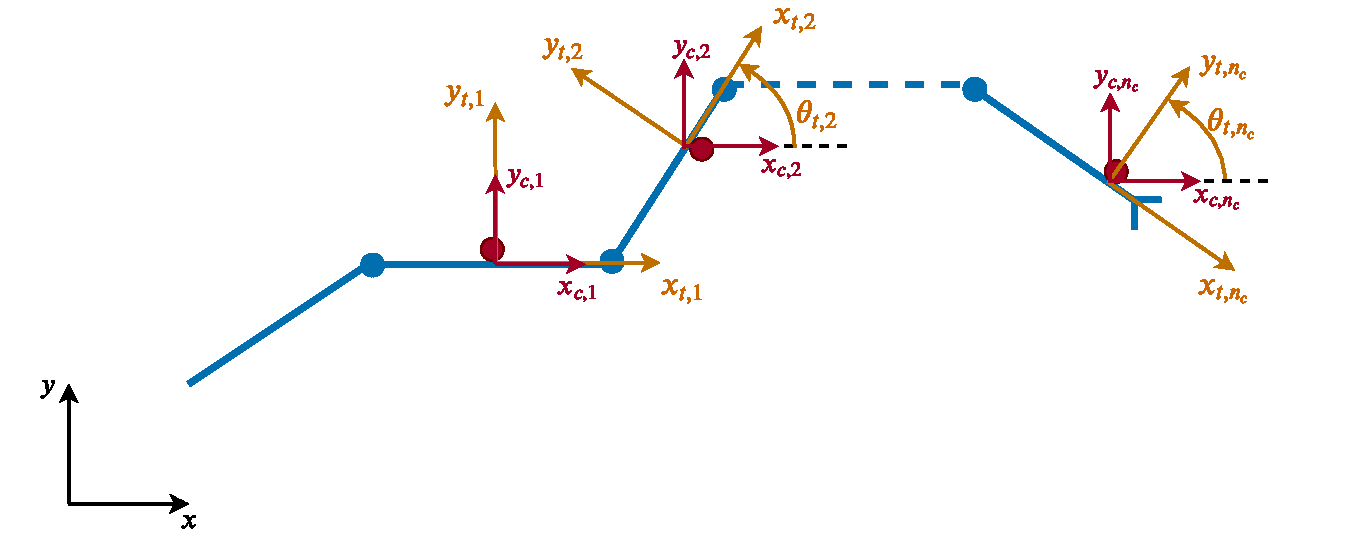
\includegraphics[width=\textwidth]{figures/theory/rt-rc.pdf}
    \caption{Model of snake robot and obstacles illustrating the task and contact frames}
    \label{fig:rt-rc}
\end{figure}


\subsubsection{Description of constraints}

In order to take the dynamics into account, the constraints are directly included into the dynamic equations of motion of the robot. This is done by expressing the constraints as a set of hypersurfaces that the robot can not physically pass. It should be noted that the focus in the paper of Yoshikawa \cite{yoshikawa1987dynamic} is on manipulator end-effector constraints and not general constraints, which should be used in the snake robot case. The constraint hypersurfaces are also expressed in the end-effector coordinates. Another important aspect of the paper is that it only addresses bilateral hypersurfaces (and not unilateral surfaces), meaning that the effector is prohibited from leaving the surface in any direction.

The $m$ hypersurfaces expressing a given constraint are given by

\begin{equation}\label{eq:hpfc:hypersurface}
    p_i(\mathbf{r}_t) = 0, \quad i = 1, 2, ..., m,
\end{equation}
\\
where $\mathbf{r}_t$ is the end effector position in a fixed reference frame. Differentiating (\ref{eq:hpfc:hypersurface}) with respect to time yields

\begin{equation}\label{eq:hpfc:derhypsurf}
    \mathbf{E}_F \mathbf{\dot{r}}_t = 0,
\end{equation}
\\
where the vectors of $\mathbf{E}_F$ are the unit normal vectors to the hypersurfaces in (\ref{eq:hpfc:hypersurface}).

By comparing the expression (\ref{eq:norm_vel5}) of the constraint on link $i$ found in \ref{seq:constraints} to (\ref{eq:hpfc:derhypsurf}), it is possible to extract the matrix $\mathbf{E}_{F,i}$ and a logical choice of $\mathbf{r}_{t,i}$ and $\mathbf{\dot{r}}_{t,i}$ presents itself.
Specifically, if one chooses

\begin{equation}
    \mathbf{r}_{t,i} =
    \begin{bmatrix}
        x_{t,i} & y_{t,i} & \theta_{t,i}
    \end{bmatrix}^T \in \mathbb{R}^3,
\end{equation}
\\
then $\mathbf{\dot{r}}_{t,i} = [\dot{x}_{t,i}, \dot{y}_{t,i}, \dot{\theta}_{t,i}]^T \in \mathbb{R}^3$ and the matrix $\mathbf{E}_{F,i}$ can by comparison be found as

\begin{equation}
    \mathbf{E}_{F,i} =
    \begin{bmatrix}
        0 & 1 & 0
    \end{bmatrix} \in \mathbb{R}^3.
\end{equation}
\\
The subscript $i$ will now be used as the constraint number, where $n_c$ is the number of constraints. This is the same as the number of contact points.
The angle $\theta_{t,i}$ of the link at the contact point is the angle $\theta$ of the link with respect to the base frame (see Figure \ref{fig:rt-rc}). It can by inspection be seen that $\mathbf{E}_{F,i}$ fulfills the criteria of being of unit size.

%These formulations do not supply an explicit expression of the corresponding constraint hypersurface. It is however not a necessity for the further computations. On the other hand it could be valuable to have the expressions for the hypersurfaces for analysis purposes.

The coordinate space $\mathbf{r}_t$ should be able to aid in expressing all the constraints present on the snake robot. Therefore, it is chosen as 

\begin{equation}
    \mathbf{r}_t = 
    \begin{bmatrix}
        \mathbf{r}_{t,1}^T & \mathbf{r}_{t,2}^T & \dots &\mathbf{r}_{t,n_c}^T
    \end{bmatrix}^T \in \mathbb{R}^{3 n_c}.
\end{equation}
\\
The same goes for $\dot{\mathbf{r}}_t$. Furthermore, the matrix $\mathbf{E}_{F}$ describing the unit normal vectors to all the hypersurfaces can now be written as

\begin{equation}
    \mathbf{E}_F = 
    \begin{bmatrix}
        \mathbf{E}_{F,1} & \mathbf{0}_{1\times3} & \dots & \mathbf{0}_{1\times3} \\
        \mathbf{0}_{1\times3} & \ddots & & \vdots \\
        \vdots & & \ddots & \mathbf{0}_{1\times3} \\
        \mathbf{0}_{1\times3} & \dots & \mathbf{0}_{1\times3} & \mathbf{E}_{F,n_c} \\
    \end{bmatrix} \in \mathbb{R}^{n_c \times 3 n_c}
\end{equation}
\\

Differentiating (\ref{eq:hpfc:derhypsurf}) further gives

\begin{equation}\label{eq:dhpfc_arf}
    \mathbf{E}_F \mathbf{\ddot{r}}_t + \mathbf{a}_{r F} = 0, \quad \mathbf{a}_{r F} = \mathbf{\dot{E}}_F\mathbf{\dot{r}}_t,
\end{equation}
\\
where the first term is believed to be the acceleration in the direction of the hypersurface, i.e. the force direction, and $\mathbf{a}_{r F} \in \mathbb{R}^{n_c}$ is believed to be an acceleration resulting from the relative movement of the task frame.

Furthermore, $\mathbf{E}_P$ is chosen so that all the vectors in the relation

\begin{equation}\label{eq:dhpfc_E}
    \mathbf{E} =
    \begin{bmatrix}
    \mathbf{E}_P \\ \mathbf{E}_F
    \end{bmatrix}
\end{equation}
\\
are mutually independent unit vectors. The matrix $\mathbf{E}_F$ represents the coordinate axes normal to the constraint surfaces, and $\mathbf{E}_P$ represents the coordinate axes complementing $\mathbf{E}_F$. Another way to display this is seeing $\mathbf{E}_F$ and $\mathbf{E}_P$ as the axes for force and position constrained directions respectively.

From the equations

\begin{equation}
    \mathbf{E\dot{r}} =
    \begin{bmatrix}
        \mathbf{E}_P \mathbf{\dot{r}}_t\\
        0
    \end{bmatrix}
    \quad \text{and} \quad
    \mathbf{E\ddot{r}}_t =
    \begin{bmatrix}
        \mathbf{E}_P \mathbf{\ddot{r}}_t \\
        -\mathbf{a}_{r F}
    \end{bmatrix}
\end{equation}
\\
it can be seen that the velocity to the constraint surface is zero, which is natural seeing as the end-effector should be physically unable to move through the surface.

For the snake robot, a simple choice of $\mathbf{E}_{P,i}$ with unit vectors complementing $\mathbf{E}_{F,i}$ is by inspection found to be

\begin{equation}\label{eq:dhpfc_EPi}
    \mathbf{E}_{P,i} = 
    \begin{bmatrix}
        1 & 0 & 0 \\
        0 & 0 & 1
    \end{bmatrix} \in \mathbb{R}^{2\times 3}.
\end{equation}
\\
This is a very logical choice, seeing as the snake robot link in contact is allowed to rotate about the obstacle and move along the obstacle.
Again, $\mathbf{E}_{P,i}$ corresponds to the $i$'th constraint. Combining all $\mathbf{E}_{P,i}$ gives 

\begin{equation}
    \mathbf{E}_P = 
    \begin{bmatrix}
        \mathbf{E}_{P,1} & \mathbf{0}_{2\times3} & \dots & \mathbf{0}_{2\times3} \\
        \mathbf{0}_{2\times3} & \ddots & & \vdots \\
        \vdots & & \ddots & \mathbf{0}_{2\times3} \\
        \mathbf{0}_{2\times3} & \dots & \mathbf{0}_{2\times3} & \mathbf{E}_{P,n_c} \\
    \end{bmatrix} \in \mathbb{R}^{2 n_c \times 3 n_c}
\end{equation}
\\
and $\mathbf{E} \in \mathbb{R}^{3 n_c \times 3 n_c}$.

%%%%%%%%%%%%%%%%%%%%%%%%%%%%%%%%%%%%%%%%%%%%%%%%%%%%%%%%%%%%%%%%%%%%%%%%%%%%%%%%%%%%%%%%%%%%%
%%%%%%%%%%%%%%%%%%%%%%%%%%%%%%%%%%%%%%%%%%%%%%%%%%%%%%%%%%%%%%%%%%%%%%%%%%%%%%%%%%%%%%%%%%%%%
%%%%%%%%%%%%%%%%%%%%%%%%%%%%%%%%%%%%%%%%%%%%%%%%%%%%%%%%%%%%%%%%%%%%%%%%%%%%%%%%%%%%%%%%%%%%%

\subsubsection{Kinematics and dynamics}

In \cite{yoshikawa1987dynamic}, the relation between the joint variable vector $\mathbf{q}$ and the end effector position $\mathbf{r}_t$ is expressed as

\begin{equation}\label{eq:hpfc:rq}
    \mathbf{r}_t = \mathbf{c(q)}.
\end{equation}
\\
The following equations are generated by differentiating \ref{eq:hpfc:rq}.

\begin{equation}
    \mathbf{\dot{r}}_t = \mathbf{J}_t \mathbf{\dot{q}}, \quad \mathbf{J}_t = \frac{\partial \mathbf{c(q)}}{\partial \mathbf{q}^T}
\end{equation}

\begin{equation}\label{eq:dhpfc_aq}
    \mathbf{\ddot{r}}_t = \mathbf{J}_t \mathbf{\ddot{q}} + \mathbf{a}_q, \quad \mathbf{a}_q = \mathbf{\dot{J}}_t \mathbf{\dot{q}}   
\end{equation}
\\
For the snake robot case, the matrix $\mathbf{J}_t$ contains the Jacobians of all the contacts.

\begin{equation}
    \mathbf{J}_t = 
    \begin{bmatrix}
        \mathbf{J}_{t,1} \\ \mathbf{J}_{t,2} \\ \vdots \\ \mathbf{J}_{t,n_c}
    \end{bmatrix} \in \mathbb{R}^{3 n_c \times N}
\end{equation}
\\
The Jacobian $\mathbf{J}_{t,i} \in \mathbb{R}^{3\times N}$ for a single contact point with respect to the contact point task variable vector $\mathbf{r}_{t,i}$ is found as 

\begin{equation}
    \mathbf{J}_{t,i} =
    \HUGE{
    \begin{bmatrix}
        \frac{\partial x_{t,i}}{\partial q_1} & \dots & \frac{\partial x_{t,i}}{\partial q_N} \\
        \frac{\partial y_{t,i}}{\partial q_1} & \dots & \frac{\partial y_{t,i}}{\partial q_N} \\
        \frac{\partial \theta_{t,i}}{\partial q_1} & \dots & \frac{\partial \theta_{t,i}}{\partial q_N}
    \end{bmatrix}
    }.
\end{equation}
\\
Furthermore, $\mathbf{a}_q \in \mathbb{R}^{n_c}$.


%%%%%%%%%%%%%%%%%%%%%%%%%%%%%%%%%%%%%%%%%%%%%%%%%%%%%%%%%%%%%%%%%%%%%%%%%%%%%%%%%%%%%%%%%%%%%
%%%%%%%%%%%%%%%%%%%%%%%%%%%%%%%%%%%%%%%%%%%%%%%%%%%%%%%%%%%%%%%%%%%%%%%%%%%%%%%%%%%%%%%%%%%%%
%%%%%%%%%%%%%%%%%%%%%%%%%%%%%%%%%%%%%%%%%%%%%%%%%%%%%%%%%%%%%%%%%%%%%%%%%%%%%%%%%%%%%%%%%%%%%

\subsubsection{Calculation of the joint driving force}

The torque resulting from the contact force is found by

\begin{equation}
    \boldsymbol{\tau}_F = \mathbf{J}_t^T \mathbf{E}_F^T \mathbf{f}_F.
\end{equation}
\\
The total torque $\boldsymbol{\tau}$ applied to the robot will be the difference between the motor torque $\boldsymbol{\tau}_c$ and the constraint torque $\boldsymbol{\tau}_F$.

\begin{equation}\label{eq:tau_dhpfc1}
    \boldsymbol{\tau} = \boldsymbol{\tau}_c - \boldsymbol{\tau}_F
\end{equation}
\\

Combining the torque in (\ref{eq:tau_dhpfc1}) with the equations of motion given in (\ref{eq:eom}) gives

\begin{equation}\label{eq:dhpfc_stuff1}
    \mathbf{M(q) \ddot{q}} + \mathbf{J}_t^T \mathbf{E}^T_F \mathbf{f}_F = \boldsymbol{\tau}_c - \mathbf{C(q, \dot{q})}
\end{equation}
\\
and
\begin{equation}\label{eq:dhpfc_stuff2}
    \mathbf{E}_F \mathbf{J}_t\mathbf{\ddot{q}} = - \mathbf{E}_F \mathbf{a}_q - \mathbf{a}_{rF}.
\end{equation}
\\
Lastly, it can be shown that combining (\ref{eq:dhpfc_stuff1}) and (\ref{eq:dhpfc_stuff2}) yields the expressions

\begin{equation}
    \mathbf{\ddot{q}} = \mathbf{M}^{-1}(\mathbf{b}_1 + (\mathbf{E}_F \mathbf{J}_t)^T \mathbf{K} (\mathbf{b}_2 - \mathbf{E}_F \mathbf{J}_t \mathbf{M}^{-1} \mathbf{b}_1)),
\end{equation}

\begin{equation}
    \mathbf{f}_F = -\mathbf{K} (\mathbf{b}_2 - \mathbf{E}_F \mathbf{J}_t \mathbf{M}^{-1} \mathbf{b}_1).
\end{equation}
\\
$\mathbf{K}$, $\mathbf{b}_1$ and $\mathbf{b}_2$ are given by

\begin{equation}
    \begin{split}
        \mathbf{K} &= (\mathbf{E}_F \mathbf{J}_t \mathbf{M}^{-1} \mathbf{J}_t^T \mathbf{E}^T_F)^{-1}\\
        \mathbf{b}_1 &= \boldsymbol{\tau}_c - \mathbf{C(q, \dot{q})}\\
        \mathbf{b}_2 &= - \mathbf{E}_F \mathbf{a}_q - \mathbf{a}_{rF}.
    \end{split}
\end{equation}
\\
Eventually, it is possible to calculate the joint control torque. It consists of a component based on the desired movement $\mathbf{\ddot{r}}_{t,d}$ in the contact point frame and a component based on the desired force $\mathbf{f}_{Fd}$ applied to the constraint surfaces. The direction of the desired force should correspond to which side of the snake robot the obstacle is. This can either be implemented into the higher level controller requesting these forces, or one could introduce a vector $\boldsymbol{\gamma}$ like in \ref{seq:constraints}. This vector consists of positive and negative units corresponding to the different obstacle placements. When multiplied with $\mathbf{f}_{Fd}$ it will simply negate the forces that should be applied to obstacles on the right side of the snake robot.

\begin{equation}\label{eq:dhpfc_tau_c}
    \boldsymbol{\tau}_c = \boldsymbol{\tau}_P + \boldsymbol{\tau}_F
\end{equation}
\\
The torque $\boldsymbol{\tau}_P$ is found by solving the equations of motion given in (\ref{eq:eom}) based on the desired values of the joint accelerations.

\begin{equation}\label{eq:dhpfc_taup}
    \boldsymbol{\tau}_P = \mathbf{M(q)} \ddot{\mathbf{q}}_d + \mathbf{C}(\mathbf{q,\dot{q}})
\end{equation}

\begin{equation}\label{eq:dhpfc_tauf}
    \boldsymbol{\tau}_F = \mathbf{J}_t^T \mathbf{E}^T_F \mathbf{f}_{Fd}
\end{equation}

\begin{equation}\label{eq:dhpfc_qddd}
    \ddot{\mathbf{q}}_d = \mathbf{J}_t^+ (\mathbf{E}^{-1} 
    \begin{bmatrix}
        \mathbf{\ddot{r}}_{EP,t,d} \\
        - \mathbf{a}_{rF}
    \end{bmatrix}
    - \mathbf{a}_q) + (\mathbf{I}-  \mathbf{J}_t^+ \mathbf{J}_t)\mathbf{k}
\end{equation}
\\
Here the vector $\mathbf{\ddot{r}}_{EP,t,d} = \mathbf{E}_P \mathbf{\ddot{r}}_{t,d}$. Furthermore, $\mathbf{J}_t^+$ denotes the pseudo inverse of the Jacobian.
The last term is included for redundant manipulators, where the vector $\mathbf{k}$ is an arbitrary time function representing the arbitrariness of the joint accelerations. It can be observed that the term $ (\mathbf{I}-  \mathbf{J}_t^+ \mathbf{J}_t)$ is the same as the projection matrix $\prescript{}{j}{\mathbf{P}}_{ap}$ onto the allowable motion space from \ref{subseq:HPFC}.

According to Yoshikawa \cite{yoshikawa1987dynamic} the position and force can be simultaneously controlled by applying the sum of the joint torque $\boldsymbol{\tau}_P$ for achieving the desired acceleration and the joint torque $\boldsymbol{\tau}_F$ for achieving the desired force as long as the robot is not in a singular state.

Describing the desired acceleration through $\mathbf{\ddot{r}}_{t,d}$ might not be the most intuitive task. It is therefore suggested that $\mathbf{E}_P$ is chosen in such a manner that a function $\mathbf{\dot{r}}_{P,t} = s(\mathbf{r}_t)$ exists and satisfies

\begin{equation}
    \mathbf{\dot{r}}_{P,t} = \mathbf{E}_P \mathbf{\dot{r}}_t.
\end{equation}
\\
If this holds, then
\begin{equation}
    \mathbf{\ddot{r}}_{P,t} = \mathbf{\ddot{r}}_{EP,t} + \mathbf{a}_{rP}, \quad \mathbf{a}_{rP} = \mathbf{\dot{E}}_P \mathbf{\dot{r}}_{P,t}.
\end{equation}
\\
Given that $\mathbf{r}_{P,t}$ is given by $\mathbf{r}_{P,t,d}$ and the described dynamics and constraints are correct, the system given by (\ref{eq:dhpfc_tau_c})-(\ref{eq:dhpfc_qddd}) will be able to realize both the desired position and force.
%%%%%%%%%%%%%%%%%%%%%%%%%%%%%%%%%%%%%%%%%%%%%%%%%%%%%%%%%%%%%%%%%%%%%%%%%%%%%%%%%%%%%%%%%%%%%
%%%%%%%%%%%%%%%%%%%%%%%%%%%%%%%%%%%%%%%%%%%%%%%%%%%%%%%%%%%%%%%%%%%%%%%%%%%%%%%%%%%%%%%%%%%%%

\section{Passive joints consideration}\label{subsec:passive-joints}

The problem that arises when computing $\boldsymbol{\tau}_P$ from (\ref{eq:dhpfc_taup}) in \ref{subsec:DHPFC}, is that the motor torques will be calculated for all joints, including the passive joints. Since the passive joints are unactuated, it is not feasible to pursue all parts of this control command. The objective is thus to change the dynamic calculations to only apply torques to the active joints. It should be noted that this challenge is more crucial for snake robots with few (active) joints. This is because a large number of active joints will dominate the control and a bigger part of the control torque can be realised.

One idea is using the dynamic coupling characteristics between the passive and active joints, as proposed by Arai et al. \cite{arai1991position}. This method assumes that there is a certain amount of active joints that can take arbitrary values determined by the other active and passive joints desired to control. That means that all joint variables still cannot be controlled to their desired values and it has to be determined which joints this should apply to. The reason for this is that the system is underactuated. A similar approach is suggested by Transeth et al. \cite{transeth2007tracking}. However this method assumes that only the active joints make out the control reference. Because it is not yet clear whether or not it will be desired to control the value of the passive joints, the rest of this section is based on the work of Arai et al. \cite{arai1991position}.

The total number of joints is now denoted $n$, whereas $r$ of these joints are active. To start off, the elements of the familiar variables $\mathbf{q}$ and $\boldsymbol{\tau}$ should be rearranged as follows

\begin{subequations}
\begin{equation}
    \mathbf{q} = 
    \begin{bmatrix}
        \boldsymbol{\phi} \\ \boldsymbol{\psi}
    \end{bmatrix}
    \begin{matrix}
        n-r\\r
    \end{matrix}
    =
    \begin{bmatrix}
        \boldsymbol{\phi} \\ \boldsymbol{\psi}_{act} \\ \boldsymbol{\psi}_{pas}
    \end{bmatrix}
    \begin{matrix}
        n-r\\2r-n \\n-r
    \end{matrix}
\end{equation}
\begin{equation}
    \boldsymbol{\tau} = 
    \begin{bmatrix}
        \boldsymbol{\tau}_{act} \\ \mathbf{0}
    \end{bmatrix}
    \begin{matrix}
        r\\n-r
    \end{matrix}.
\end{equation}
\end{subequations}
\\
Here $\boldsymbol{\psi}$ are the $r$ joint variables, both passive and active, that will be controlled to their desired value. $\boldsymbol{\phi}$ contains the remaining $n-r$ active joint values. Furthermore, the corresponding generalized force vector $\boldsymbol{\tau}$ is divided into an active and a passive part. The part corresponding to the passive joints is zero because the generalized forces on the passive joints by definition are zero.

The inertia and Coriolis matrices $\mathbf{M(q)}$ and $\mathbf{C(q,\dot{q})}$ can now be rearranged accordingly.

\begin{subequations}
\begin{equation}\label{eq:pas-M}
    \mathbf{M(q)} =
    \underset{n-r\quad\quad\quad r}{\begin{bmatrix}
        \mathbf{M}_{11}(\mathbf{q}) & \mathbf{M}_{12}(\mathbf{q})\\
        \mathbf{M}_{21}(\mathbf{q}) & \mathbf{M}_{22}(\mathbf{q})
    \end{bmatrix}}
    \begin{matrix}
        r\\n-r
    \end{matrix}
\end{equation}
\begin{equation}\label{eq:pas-C}
    \mathbf{C(q,\dot{q})} =
    \begin{bmatrix}
        \mathbf{C}_1(\mathbf{q,\dot{q}})\\
        \mathbf{C}_2(\mathbf{q,\dot{q}})
    \end{bmatrix}
    \begin{matrix}
        r\\n-r
    \end{matrix}
\end{equation}
\end{subequations}
\\
Using (\ref{eq:pas-M}) and (\ref{eq:pas-C}), the equations of motion (\ref{eq:eom}) can be split into two separate equations.

\begin{subequations}
\begin{equation}\label{eq:pas-eom-1}
    \mathbf{M}_{11} \ddot{\boldsymbol{\phi}} + \mathbf{M}_{12} \ddot{\boldsymbol{\psi}} + \mathbf{C}_1 = \boldsymbol{\tau}_{act}
\end{equation}
\begin{equation}\label{eq:pas-eom-2}
    \mathbf{M}_{21} \ddot{\boldsymbol{\phi}} + \mathbf{M}_{22} \ddot{\boldsymbol{\psi}} + \mathbf{C}_2 = \mathbf{0}
\end{equation}
\end{subequations}
\\
When the values for $\mathbf{q}$ and $\dot{\mathbf{q}}$ are inserted and the desired values $\ddot{\boldsymbol{\psi}}_d$ are assigned to the accelerations $\ddot{\boldsymbol{\psi}}$, (\ref{eq:pas-eom-2}) is considered a linear equation with regard to $\ddot{\boldsymbol{\phi}}$. The coefficient matrix $\mathbf{M}_{21}$ corresponds to the dynamic coupling between the accelerations of $\boldsymbol{\phi}$ and the generalized forces of the passive joints, and it depends upon the structure and mass distribution of the manipulator \cite{arai1991position}.

Solving (\ref{eq:pas-eom-2}) for $\ddot{\boldsymbol{\phi}}$ yields

\begin{equation}\label{eq:pas-phidd}
    \ddot{\boldsymbol{\phi}} = - \mathbf{M}^{-1}_{21}  \mathbf{M}_{22} \ddot{\boldsymbol{\psi}}_d - \mathbf{M}^{-1}_{21} \mathbf{C}_2.
\end{equation}
\\
This is given that the matrix $\mathbf{M}_{21}$ is nonsingular. Arai et al. \cite{arai1991position} proved that this is also the condition for output controllability.
The generalized forces on the active joints can be found by substituting (\ref{eq:pas-phidd}) into (\ref{eq:pas-eom-1}).

\begin{equation}\label{eq:tau-act}
    \boldsymbol{\tau}_{act} = (\mathbf{M}_{12} - \mathbf{M}_{11} \mathbf{M}^{-1}_{21} \mathbf{M}_{22})\ddot{\boldsymbol{\psi}}_d + \mathbf{C}_1 - \mathbf{M}_{11} \mathbf{M}^{-1}_{21} \mathbf{C}_2
\end{equation}
\\
If the generalized forces $\boldsymbol{\tau}_{act}$ are applied to the active joints, the resulting accelerations will be $\ddot{\boldsymbol{\phi}}$ and $\ddot{\boldsymbol{\psi}}_d$ \cite{arai1991position}.

From the dimensions of $\boldsymbol{\phi}$ and $\boldsymbol{\psi}$ it can be deduced that if the number of active joints $r$ equals the total number of joints $n$, all joint variables can be controlled. This is what would be referred to as a fully actuated system. If, on the other hand, there were no active joints, the dimension of $\boldsymbol{\psi}$ would be zero and all variables would be uncontrollable. These two cases are both quite intuitive. The more vital question is exactly how many of the joints are required to be active in order to achieve the desired control goal. This is equivalent to the question of how many of the joint variables are desired to be controlled, and is dependent on the full HOAL algorithm.

Seeing as the joints desired to be controlled will change continuously for a snake robot traversing a terrain with obstacles, this is probably not the most robust solution. The bottom line is however that the control torques are mapped to the active joints and all of them can now be commanded to the snake robot. The method is tested in \ref{sec:pas-pos} and further discussed in \ref{subsec:dis-passive-joints}.
%%%%%%%%%%%%%%%%%%%%%%%%%%%%%%%%%%%%%%%%%%%%%%%%%%%%%%%%%%%%%%%%%%%%%%%%%%%%%%%%%%%%%%%%%%%%%
%%%%%%%%%%%%%%%%%%%%%%%%%%%%%%%%%%%%%%%%%%%%%%%%%%%%%%%%%%%%%%%%%%%%%%%%%%%%%%%%%%%%%%%%%%%%%

\section{The utility of dynamic HPFC in snake robot locomotion}

Most of the snake robot locomotion strategies today are intended for flat surfaces. Lateral undulation and sidewinding are two of these strategies presented in \ref{subsec:traditional-loco}. Even though they are based on flat surfaces, they require some amount of ground friction to yield propulsion. Either way, the snake robot body motions are the basis for the propulsion. A position controller for the joint angles of the snake robot would thus induce a satisfying behavior. Consequently, a hybrid position/force controller would simply be an overkill for these strategies. The concertina locomotion strategy, on the other hand, is conducted in narrow spaces where the snake robot anchors itself against the environment. This is also explained further in \ref{subsec:traditional-loco}. A joint controller is sufficient in this case as well if only the curling up and stretching out of the robot is considered. It might however be desired for the snake robot to push against its environment at the same time as this movement takes place. A hybrid position force controller could then be useful to simultaneously realize these control goals.

Compliance control, presented in \ref{subsec:compliance-control}, is another control option for adapting to the environment. The main difference between compliance control and dynamic HPFC is that the compliance controller is a so called reactive controller, meaning that the robot will change its curvature according to the environment when a contact feedback has been received. The dynamic HPFC contrarily uses a feedforward term for dynamic force, enabling it to always control both the force and position precisely. The success of this method does to a large degree depend on a correct modeling of the dynamics of the robot and its environment.

The locomotion method which can take the most advantage of the dynamic HPFC is the OAL method presented in \ref{subsec:OAL}. The possibility to control position and force simultaneously and independently in different directions allows the snake robot to both move between obstacles and push against them at the same time. Furthermore, the dynamical control facilitates a dynamical or compliant, rather than stiff, behavior. This is beneficial for the mechanical parts of the snake robot which can then experience a lower level of strain and wear and tear. 


%Give a brief overview of the most important strategies for terrestrial snake robot locomotion, and discuss the prospective properties of HPFC in the context of your findings.

%- Controlling both the force and position using compliance control would require us to frequently switch between very very high and very low compliance. Det er vel directional compliance tho

%- vi likevel ha en viss compliant behavior i at hvis en hindring beveger seg litt vil slangen følge etter --> men det kan være en assumption at hindringene har statisk posisjon

%- posisjonsstyring gir stiv oppførsel og krafstyring gir dynamisk oppførsel

%%%%%%%%%%%%%%%%%%%%%%%%%%%%%%%%%%%%%%%%%%%%%%%%%%%%%%%%%%%%%%%%%%%%%%%%%%%%%%%%%%%%%%%%%%%%%
%%%%%%%%%%%%%%%%%%%%%%%%%%%%%%%%%%%%%%%%%%%%%%%%%%%%%%%%%%%%%%%%%%%%%%%%%%%%%%%%%%%%%%%%%%%%%
%%%%%%%%%%%%%%%%%%%%%%%%%%%%%%%%%%%%%%%%%%%%%%%%%%%%%%%%%%%%%%%%%%%%%%%%%%%%%%%%%%%%%%%%%%%%%

\section{Application challenges related to dynamic HPFC}

There are surely several ways of implementing and designing the dynamic HPFC control logic on a snake robot. This section will focus on the challenges related to the application of the suggested design scheme in \ref{subsec:DHPFC}. Special attention is paid to the chosen variable spaces and the consequences of configuration transitions when the snake robot moves.

\subsection{Computational challenges}

Whenever the snake robot achieves successful forward or backward propulsion it will slide along the obstacles that are by its side. Eventually the contact between a given link and an obstacle will be lost. At this point, the obstacle will either be left alone or come in contact with a neighboring link. These two scenarios are illustrated in Figures \ref{fig:obst_slide_seq1} and \ref{fig:obst_slide_seq2} respectively. If the contact is completely lost, it means that one constraint is lost as well and $n_c = n_c - 1$. This will in turn lead to the variable $\mathbf{r}_t$, describing the position of the contacts, shrinking. Consequently the mapping matrix $\mathbf{E}$ to the allowed force and movement directions will shrink as well. The most significant challenge in this case is changing the dimensions of the affected variables in real-time. One option could be keeping all variable spaces unchanged and instead set the parts of $\mathbf{E}$ corresponding to the lost constraint to zero so that it has no impact on the following solution.

\begin{figure}[h!]
    \centering
    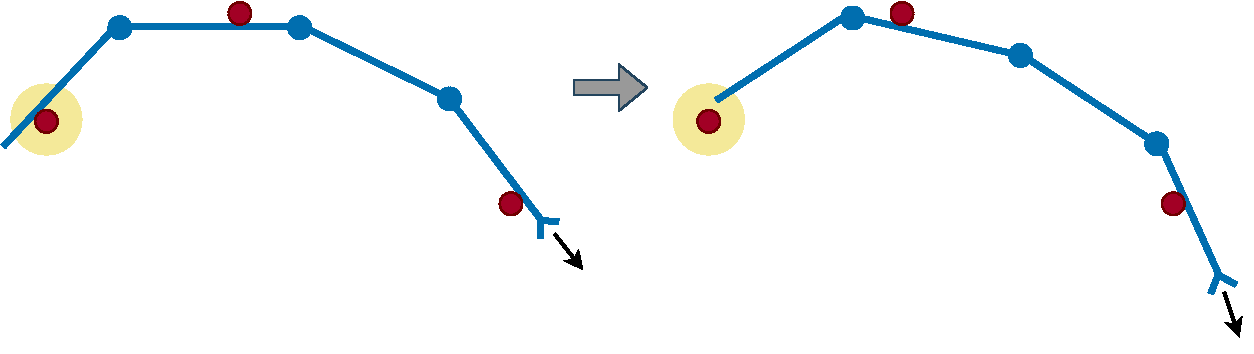
\includegraphics[width=\textwidth]{figures/theory/obst_slide_sequence1.pdf}
    \caption{Snake robot losing contact with obstacle}
    \label{fig:obst_slide_seq1}
\end{figure}

\begin{figure}[h!]
    \centering
    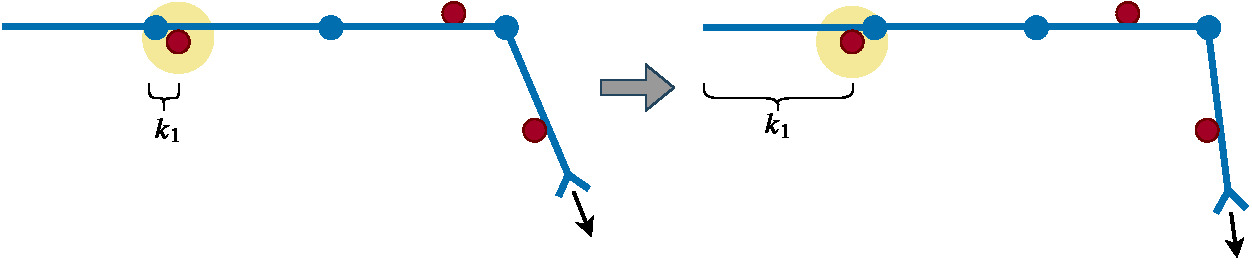
\includegraphics[width=\textwidth]{figures/theory/obst_slide_sequence2.pdf}
    \caption{Obstacle changing contact from one link to another}
    \label{fig:obst_slide_seq2}
\end{figure}

If, on the other hand, the snake simply slides in a way that the contact is transferred to an adjoining link, the size $n_c$ and dimensions of all variables will remain unchanged. In addition to this, the obstacle will lie on the same side of the snake as it already was, which enables the direction of the desired force application to the obstacle to stay the same. Thus, the constraint will generally be on the same form. The only thing that has to change is the description of the position variables in $\mathbf{r}_t$ belonging to the new contact point. Again, the change is most probably slim since the two first variables $(x_t, y_t)$ describe the position of the contact point, and the obstacle is assumed to be static (meaning its position will not change even though the calculation of the position changes). Furthermore, the adjoining link adopting the contact is probable to have a similar angle $\theta_t$ relative to the base frame as the previous link given that the desired path is well designed and defined. From this it follows that the joint variable $\phi_c$ back to the obstacle frame will stay similar to what it was as well. These aspects obviously make the implementation simpler and the control sequence smoother and more predictable.

Even though the numerical value of the mentioned variables do not change drastically, the Jacobian will have to be recalculated since the variables now are described by a new subset of the joint variables. Finding a new expression for the Jacobian matrix and its derivative in real-time is not a trivial, nor fast, operation. One option would of course be pre-computing $\mathbf{J}$ and $\dot{\mathbf{J}}$ for every link that could be in contact with an obstacle and only employ the ones that are relevant at the specific time instance. There is however still a challenge related to this case. The generalized joint variables $\mathbf{q}$ contain the distances $k$ from the contact points to the preceding joints. It is important that these distances are not mixed and that they are only used once. In other words, two contact points should not be described by the same $k$. As a consequence of this, the Jacobian for every link would have to be computed with all the possible $k$'s. Logically, this would in turn lead to a large number of pre-computed matrices as the number of links and obstacles grow. In addition to this, the right set of Jacobians would have to be chosen in real-time while administering that they all use unique $k$'s. This should be done without changing the existing setup more than necessary in order to avoid jumps in the control. It is very much an achievable task, but at the same time an extra challenge.

With a contact moving from one link to another, the corresponding joint variable $k$ describing the position of the contact point will change and the manner in which it is computed will also change. This is once again an achievable, yet challenging task to perform in real-time. It should also be noted that the value of this $k$ will probably experience a jump. This is because the contact moves from the end of a link to the beginning of a link, or vice versa, and the distance is always measured with respect to the preceding joint of the link in contact. This is illustrated in Figure \ref{fig:obst_slide_seq2}. On the other hand, it is reassuring that the matrices $\mathbf{M(q)}$ and $\mathbf{C(q,\dot{q})}$ are unaltered by the change of a $k$. This is logical since these matrices describe the dynamics of the snake robot alone.

The biggest challenge arises if the number of contact points increase. This means that the dimension of all variables will have to increase correspondingly and the Jacobians have to be either re-computed or re-assembled. It is in this case important to keep in mind the challenge associated with memory allocation in the software being used.

\subsection{Differences with the traditional manipulator case}

One significant challenge related to snake robots as opposed to traditional robot manipulators is the presence of passive joints at the base of the robot. The passive joints of the snake robot that are attached to the base frame, $[\phi_0, x_0, y_0]$ are included in the description of the position of every link and contact point. This means that if they were actuated, they could have influenced all the points that are desired to control, given that the robot is not stuck between obstacles. The dynamic hybrid position/force controller could therefore introduce a desired joint acceleration value $\ddot{\mathbf{q}}_d$ for these passive joints when recalculating from the desired contact point accelerations $\ddot{\mathbf{r}}_{t,d}$. Since these joints are passive, they are also uncontrollable and a desired control input on the joints is not realizable. A greater number of joints will generally make this challenge less significant because it leads to a larger degree of controllability of all contact points.

When it comes to the assignments of traditional robot manipulators and snake robots, they are usually a lot more repetitive and pre-defined for robot manipulators. A typical task for an industrial hybrid position force controlled robot manipulator is polishing a known surface with a given pressure. An example is given in Figure \ref{fig:robotman-polish}. The snake robot might also be familiar with the shape of its current environment, but this is something that is constantly changing as the robot moves through the world. Thus, the position and force application requirements are constantly changing as well. Furthermore, since the snake robot is eventually meant to locomote through outdoor environments, it will encounter different kinds of obstacles as illustrated in Figure \ref{fig:weird-env}. They can differ in both size and texture, and be either soft or rigid. Thus, there are a lot of factors the snake robot will have to take into account. For this project however, the environment and control goals are significantly simplified.

\begin{figure}
    \centering
    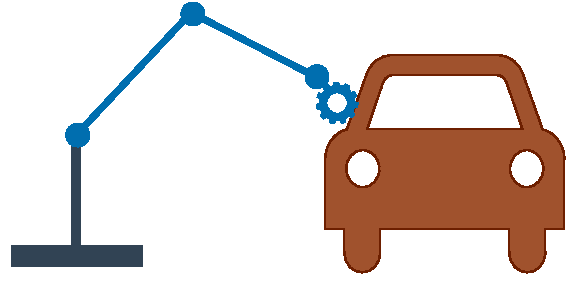
\includegraphics[width=0.6\textwidth]{figures/theory/robotman-polish.pdf}
    \caption{Industrial robot manipulator polishing a car}
    \label{fig:robotman-polish}
\end{figure}

\begin{figure}
    \centering
    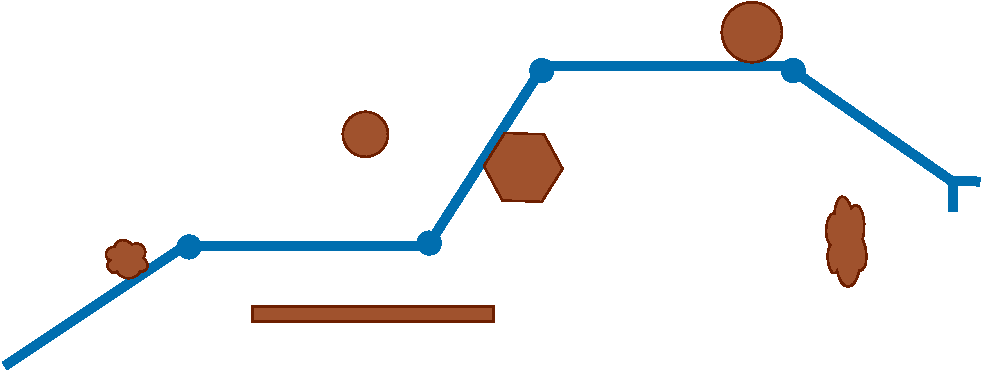
\includegraphics[width=0.7\textwidth]{figures/theory/weird-environment.pdf}
    \caption{Snake robot in environment with varying obstacle types}
    \label{fig:weird-env}
\end{figure}

There is also a considerable difference in the typical constraints on a snake robot and a traditional manipulator. Manipulators usually only have constraints or obstacles in the close environment of the end effector in which the manipulator is performing a task. It might also have some limitations regarding the motion span of its joints, but this applies to snake robots as well, though perhaps to a smaller degree. The environment the snake robot is traversing may as mentioned contain various and spread out obstacles, making the constraints different from time to time. If, however, a robot is in an undesirable position between obstacles, a snake robot might have an advantage in that it can exit its current configuration from several different directions since no part of it is fixed to any point in the world.

%- Arbitrary number of obstacles and constantly changing requirements (desired force application etc, as opposed to a typical industrial manipulator that simply should polish a surface with a given pressure repeatedly)

%- The environment is constantly changing and the contact wont be a point contact in the real world, and the snake robot might encounter all kinds of surfaces and textures (rigid, soft, slippery etc)
%%%%%%%%%%%%%%%%%%%%%%%%%%%%%%%%%%%%%%%%%%%%%%%%%%%%%%%%%%%%%%%%%%%%%%%%%%%%%%%%%%%%%%%%%%%%%
%%%%%%%%%%%%%%%%%%%%%%%%%%%%%%%%%%%%%%%%%%%%%%%%%%%%%%%%%%%%%%%%%%%%%%%%%%%%%%%%%%%%%%%%%%%%%

%
\subsection{Example of dynamic HPFC on simple snake robot}

This section shows a very simple scenario with a 2-link robot and one obstacle. The aim is to provide a better understanding of the theory presented in \ref{subsec:DHPFC} and show the structure of the various mapping matrices.
Furthermore, the example shows the necessity of using simulation software to study more intricate cases, as the matrices for this simple case already get quite complex.

The configuration of the robot and its environment is illustrated in Figure \ref{fig:ex_2link}. %To make the example as simple as possible, the robot is still in the given configuration and all velocities are thus zero.
The mass of each link is $m = 1 kg$ and the link length is $l=1 m$. The value of the joint angles $\phi_0$ and $\phi_1$ are $0$ and $\pi/2$ respectively.

\begin{figure}
    \centering
    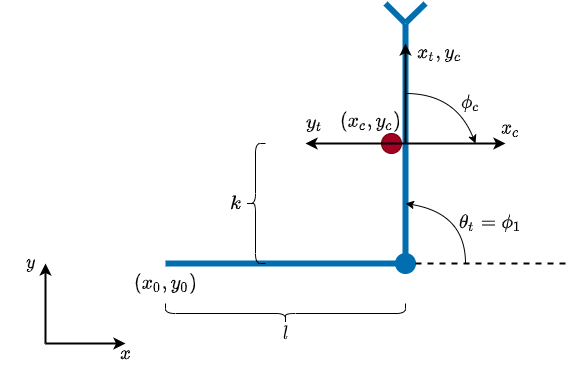
\includegraphics[width=0.9\textwidth]{figures/theory/example_2link.png}
    \caption{Model of 2-link snake robot}
    \label{fig:ex_2link}
\end{figure}

The joint variables are given by

\begin{equation}
    \mathbf{q} =
    \begin{bmatrix}
        \phi_0 & \phi_1 & x_0 & y_0 & k & \phi_c
    \end{bmatrix}^T \in \mathcal{R}^5.
\end{equation}
\\
The task coordinates by the contact point are given by

\begin{equation}
    \mathbf{r}_t = 
    \begin{bmatrix}
        x_c & y_c & \theta_t
    \end{bmatrix}^T \in \mathcal{R}^3,
\end{equation}
\\
where $\theta_t$ in the given configuration is the sum of the two joint angles $\phi_0$ and $\phi_1$. Furthermore, the constraint coordinates, which should always remain constant, are given by

\begin{equation}
    \mathbf{r}_c = 
    \begin{bmatrix}
        x_c & y_c & \theta_c
    \end{bmatrix}^T \in \mathcal{R}^3,
\end{equation}
\\
where $\theta_c$ is the angle of the obstacle point coordinate system in the base frame. This angle should always be zero, as can be seen from Figure \ref{fig:ex_2link}. It should be noted that the origin of the two frames, described by $(x_c, y_c)$, is the same. This is a result of the contact point and obstacle being modeled as a single point.

Lastly, the velocities and forces represented in the task frame (visualized in Figure \ref{fig:ex_2link} as $(x_t, y_t)$) are 

\begin{equation}
    \mathbf{v} =
    \begin{bmatrix}
        v_x & v_y
    \end{bmatrix}^T \in \mathcal{R}^2,
\end{equation}

\begin{equation}
    \mathbf{f} =
    \begin{bmatrix}
        f_x & f_y
    \end{bmatrix}^T \in \mathcal{R}^2.
\end{equation}
\\

\subsubsection{Dynamics}

The dynamics of this robot can be found using the Euler-Lagrange method described in \ref{sec:dyn}.
The position and velocities of the middle of the links in the base frame are

\begin{equation}
    \begin{split}
        p_0 &=
        \begin{bmatrix}
            x_0 + l/2 cos(\phi_0)\\
            y_0 + l/2 sin(\phi_0)
        \end{bmatrix}, \\
        p_1 &=
        \begin{bmatrix}
            x_0 + l cos(\phi_0) + l/2 cos(\phi_0+ \phi_1)\\
            y_0 + l sin(\phi_0) + l/2 sin(\phi_0+\phi_1)
        \end{bmatrix},
    \end{split}
\end{equation}

\begin{equation}
    \begin{split}
        \dot{p}_0 &=
        \begin{bmatrix}
            \dot{x_0} - l/2 \dot{\phi_0} sin(\phi_0)\\
            \dot{y_0} + l/2 \dot{\phi_0} cos(\phi_0)
        \end{bmatrix}, \\
        \dot{p}_1 &=
        \begin{bmatrix}
            \dot{x_0} - l \dot{\phi_0} sin(\phi_0) - l/2 (\dot{\phi}_0 +\dot{\phi}_1) sin(\phi_0+\phi_1)\\
            \dot{y_0} + l \dot{\phi_0} cos(\phi_0) + l/2 (\dot{\phi}_0 +\dot{\phi}_1) cos(\phi_0+\phi_1)
        \end{bmatrix}.
    \end{split}
\end{equation}
\\
The Lagrangian and the dynamical equations can now be calculated from (\ref{eq:ex_dyn1}) and (\ref{eq:ex_dyn2}), where $I = (1/12)ml^2 = 1/12$.

\begin{equation}\label{eq:ex_dyn1}
    \begin{split}
        L &= K_{translational,0} + K_{rotational,0} + K_{translational,1} + K_{rotational,1}\\
        &= \frac{1}{2} m \dot{p}_0^2 + \frac{1}{2}I\dot{\phi_0}^2 + \frac{1}{2} m \dot{p}_1^2 + \frac{1}{2}I\dot{\phi_1}^2
    \end{split}
\end{equation}
\\
\begin{equation}\label{eq:ex_dyn2}
    \boldsymbol{\tau} = \frac{d}{dt} \frac{\partial L}{\partial \dot{\mathbf{q}}} - \frac{\partial L}{\partial \mathbf{q}}
\end{equation}
\\
Inserting the values for the constants $m$ and $l$ and comparing the result to the form given in (\ref{eq:eom}) gives the inertia and Coriolis matrix in (\ref{eq:ex_inertia}) and (\ref{eq:ex_coriolis}) respectively. The trigonometric functions are abbreviated to $s_0 = sin(\phi_0)$, $s_1 = sin(\phi_1)$, $c_0 = cos(\phi_0)$, $c_1 = cos(\phi_1)$, $s_{01} = sin(\phi_0+\phi_1)$ and $c_{01} = cos(\phi_0+\phi_1)$.

\begin{equation}\label{eq:ex_inertia}
    \mathbf{M(q)} = 
    \begin{bmatrix}
        c_1+\frac{5}{3} & \frac{c_1}{2} + \frac{1}{3} & -\frac{s_{01}}{2} - \frac{3s_0}{2} & \frac{c_{01}}{2} + \frac{3c_0}{2} & 0 & 0 \\
        \frac{c_1}{2}+\frac{1}{3} & \frac{1}{3} & -\frac{s_{01}}{2} & \frac{c_{01}}{2} & 0 & 0 \\
        -\frac{s_{01}}{2}- \frac{3s_0}{2} & -\frac{s_{01}}{2} & 2 & 0 & 0 & 0 \\
        \frac{c_{01}}{2}+ \frac{3c_0}{2} & \frac{c_{01}}{2} & 0 & 2 & 0 & 0 \\
        0 & 0 & 0 & 0 & 0  & 0 \\
        0 & 0 & 0 & 0 & 0  & 0
    \end{bmatrix}
\end{equation}

\begin{equation}\label{eq:ex_coriolis}
    \mathbf{C(q, \dot{q})} = 
    \begin{bmatrix}
        -\frac{\dot{\phi}_1 s_1 (2\dot{\phi}_0+ \dot{\phi}_1)}{2} \\
        \frac{\dot{\phi}_0^2 s_1}{2} \\
        -\frac{3 \dot{\phi}_0^2 c_1}{2} - \frac{\dot{\phi}_0^2 c_{01}}{2} - \frac{\dot{\phi}_1^2 c_{01}}{2} - \dot{\phi}_0 \dot{\phi}_1 c_{01} \\
        -\frac{3 \dot{\phi}_0^2 s_1}{2} - \frac{\dot{\phi}_0^2 s_{01}}{2} - \frac{\dot{\phi}_1^2 s_{01}}{2} - \dot{\phi}_0 \dot{\phi}_1 s_{01} \\
        0 \\ 0
    \end{bmatrix}
\end{equation}
\\
Inserting the given angles significantly simplifies the matrices to

\begin{equation}
    \mathbf{M} = 
    \begin{bmatrix}
        5/3 & 1/3 & -1/2 & 3/2 & 0& 0 \\
        1/3 & 1/3 & -1/2 & 0 & 0 & 0\\
        -1/2 & -1/2 & 2 & 0 & 0 & 0\\
        3/2 & 0 & 0 & 2 & 0 & 0\\
        0 & 0 & 0 & 0 & 0 & 0\\
        0 & 0 & 0 & 0 & 0 & 0
    \end{bmatrix}
\end{equation}

\begin{equation}
    \mathbf{C(\dot{q})} = 
    \begin{bmatrix}
        -(\dot{\phi}_1 (2\dot{\phi}_0+ \dot{\phi}_1))/2 \\
        \dot{\phi}_0^2/2 \\
        0 \\
        -3 \dot{\phi}_0^2/2 - \dot{\phi}_0^2/2 - \dot{\phi}_1^2/2 - \dot{\phi}_0 \dot{\phi}_1 \\
        0 \\ 0
    \end{bmatrix}.
\end{equation}

\subsubsection{Constraints}

The single obstacle present in this example stands for the single constraint on the snake robot. 
From \ref{subsec:DHPFC} it is known that the constraint is on the velocity of the contact point normal to the link in contact. This velocity is here given as

\begin{equation}
    v_y = - sin(\theta_t) \dot{x}_c + cos(\theta_t) \dot{y}_c
\end{equation}
\\
In order for the link to both stick to the obstacle and not penetrate it, the velocity $v_y$ should be zero. This constraint is put on the form in (\ref{eq:hpfc:derhypsurf}) and the given angles are inserted.

\begin{equation}\label{eq:ex_EF}
    \mathbf{E}_F = 
    \begin{bmatrix}
        - sin(\theta_t) & cos(\theta_t) & 0
    \end{bmatrix}
    =
    \begin{bmatrix}
        - 1 & 0 & 0
    \end{bmatrix}
\end{equation}
\\
The derivative of (\ref{eq:ex_EF}) is
\begin{equation}\label{eq:ex_EFd}
    \mathbf{\dot{E}}_F = 
    \begin{bmatrix}
        -cos(\theta_t) \dot{\theta}_t & - sin(\theta_t) \dot{\theta}_t & 0
    \end{bmatrix}
    \begin{bmatrix}
        0 & -\dot{\theta}_t & 0
    \end{bmatrix}.
\end{equation}
\\
Inserting (\ref{eq:ex_EFd}) into (\ref{eq:dhpfc_arf}) gives
\begin{equation}
    a_{rF} = -\dot{\theta}_t \dot{y}_c.
\end{equation}
\\
It is however known that the obstacle itself cannot move. This, together with the obstacle being modeled as a point, results in the velocity of the contact point being zero at all times. Thus $a_{rF}=0$.

(\ref{eq:dhpfc_EPi}) and (\ref{eq:dhpfc_E}) give
\begin{equation}
    \mathbf{E}_P = 
    \begin{bmatrix}
        cos(\theta_t) & sin(\theta_t) & 0 \\
        0 & 0 & 1
    \end{bmatrix}=
    \begin{bmatrix}
        0 & 1 & 0 \\
        0 & 0 & 1
    \end{bmatrix},
\end{equation}
\begin{equation}
    \mathbf{E}=
    \begin{bmatrix}
        0 & 1 & 0 \\
        0 & 0 & 1 \\
        -1 & 0 & 0
    \end{bmatrix}.
\end{equation}
\\
The task coordinates can be expressed as
\begin{equation}
    \mathbf{r}_t =
    \begin{bmatrix}
        x_0 + l cos(\phi_0) + k cos(\phi_0+\phi_1)\\
        y_0 + l sin(\phi_0) + k sin(\phi_0+\phi_1)\\
        \phi_0+\phi_1
    \end{bmatrix}.
\end{equation}
\\
The corresponding Jacobian an its derivative can thus be calculated to
\begin{equation}
    \begin{split}
        \mathbf{J}_t&=
        \begin{bmatrix}
            -l s_0 - k s_{01} & - k s_{01} & 1 & 0 & c_{01} & 0 \\
            l c_0 + k c_{01} & k c_{01} & 0 & 1 & s_{01} & 0 \\
            1 & 1 & 0 & 0 & 0 & 0
        \end{bmatrix}\\&=
        \begin{bmatrix}
            - k & - k & 1 & 0 & 0 & 0 \\
            1 &0 & 0 & 1 & 1 & 0 \\
            1 & 1 & 0 & 0 & 0 & 0
        \end{bmatrix},
    \end{split}
\end{equation}
\begin{equation}\label{eq:ex_Jd}
    \begin{split}
        \mathbf{\dot{J}}_t&=
        \begin{bmatrix}
            - \dot{k} s_{01} -l \dot{\phi}_0c_0 -k c_{01}(\dot{\phi_0}+\dot{\phi_1}) & -\dot{k} s_{01}-k c_{01}(\dot{\phi_0}+\dot{\phi_1}) & 0 & 0 & -s_{01}(\dot{\phi_0}+\dot{\phi_1})  & 0\\
            \dot{k} c_{01} -l \dot{\phi}_0s_0 -k s_{01}(\dot{\phi_0}+\dot{\phi_1}) & \dot{k} c_{01}-k s_{01}(\dot{\phi_0}+\dot{\phi_1}) & 0 & 0 & c_{01}(\dot{\phi_0}+\dot{\phi_1}) & 0 \\
            0 & 0 & 0 & 0 & 0 & 0
        \end{bmatrix}\\&=
        \begin{bmatrix}
            - \dot{k} -\dot{\phi}_0 & -\dot{k} & 0 & 0 & -(\dot{\phi_0}+\dot{\phi_1}) & 0 \\
            -\dot{k}(\dot{\phi_0}+\dot{\phi_1}) & -\dot{k}(\dot{\phi_0}+\dot{\phi_1}) & 0 & 0 & 0 & 0\\
            0 & 0 & 0 & 0 & 0 & 0
        \end{bmatrix}.
    \end{split}
\end{equation}
\\
Inserting (\ref{eq:ex_Jd}) into (\ref{eq:dhpfc_aq}) gives
\begin{equation}
    \mathbf{a}_q =
    \begin{bmatrix}
            - (\dot{k} +\dot{\phi}_0)\dot{\phi}_0 -\dot{k} \dot{\phi}_1 -(\dot{\phi_0}+\dot{\phi_1})\dot{k} \\
            -\dot{k}(\dot{\phi_0}+\dot{\phi_1})\dot{\phi}_0 -\dot{k}(\dot{\phi_0}+\dot{\phi_1})\dot{\phi}_1 \\
            0
        \end{bmatrix}.
\end{equation}

\subsubsection{Calculation of the control torque}

All matrices necessary to derive the control torque are now defined. To make the calculation of the torque even simpler, the static case where all velocities are zero is considered. The result is calculated using (\ref{eq:dhpfc_tau_c})-(\ref{eq:dhpfc_qddd}) and a desired force $f_F = 1 N$ and desired acceleration $\ddot{\mathbf{r}}_d = [0, 0, 1 rad/s^2]^T$. \hl{Quite fast rotation and light force?}

\begin{equation}
    \mathbf{\ddot{q}}_d =
    \begin{bmatrix}
        0 & \frac{1}{5} & \frac{2}{5}\\
        0 & -\frac{1}{5} & \frac{3}{5}\\
        1 & 0 & k \\
        0 & \frac{2}{5} & -\frac{1}{5}\\
        0 & \frac{2}{5} & -\frac{1}{5} \\
        0 & 0 & 0
    \end{bmatrix}\left\{
    \begin{bmatrix}
        0 & 0 & -1\\
        1 & 0 & 0\\
        0 & 1 & 0
    \end{bmatrix}
    \begin{bmatrix}
        0\\   1\\   0
    \end{bmatrix}-
    \begin{bmatrix}
        0\\   0\\   0
    \end{bmatrix}\right\}=
    \begin{bmatrix}
        \frac{2}{5}\\
        \frac{3}{5}\\
        k \\
        -\frac{1}{5}\\
        -\frac{1}{5} \\
        0
    \end{bmatrix}
\end{equation}
\\
The distance $k$ from the joint to the obstacle is chosen to be $1/2 m$.
\begin{equation}
    \boldsymbol{\tau}_P = 
    \begin{bmatrix}
        5/3 & 1/3 & -1/2 & 3/2 & 0 & 0 \\
        1/3 & 1/3 & -1/2 & 0 & 0 & 0 \\
        -1/2 & -1/2 & 2 & 0 & 0 & 0 \\
        3/2 & 0 & 0 & 2 & 0 & 0 \\
        0 & 0 & 0 & 0 & 0  & 0\\
        0 & 0 & 0 & 0 & 0  & 0
    \end{bmatrix}
    \begin{bmatrix}
        2/5\\
        3/5\\
        k \\
        -1/5\\
        -1/5\\0
    \end{bmatrix}=
    \begin{bmatrix}
        0.3167\\
        0.0833\\
        0.5000 \\
        0.2000\\
        0\\0
    \end{bmatrix}
\end{equation}

\begin{equation}
    \boldsymbol{\tau}_F = 
    \begin{bmatrix}
       -k & 1 & 1\\
       -k & 0 & 1\\
       1 & 0 & 0\\
       0 & 1 & 0\\
       0 & 1 & 0 \\
       0 & 0 & 0
    \end{bmatrix}
    \begin{bmatrix}
        -1 \\ 0 \\ 0
    \end{bmatrix}=
    \begin{bmatrix}
       0.5000\\
       0.5000\\
       -1.000\\
       0.000\\
       0.000\\ 0
    \end{bmatrix}
\end{equation}

\begin{equation}
    \boldsymbol{\tau}_c =
    \begin{bmatrix}
        0.8167 & 0.5833 & -0.5000 & 0.2000 & 0.000 & 0.000
    \end{bmatrix}^T
\end{equation}

\hl{Discuss this result. The torques to the translational positions cannot be applied. Is this what the servo feedback thing is for?? only tau 1 can really be applied. k ends up being a free variable!}

%%%%%%%%%%%%%%%%%%%%%%%%%%%%%%%%%%%%%%%%%%%%%%%%%%%%%%%%%%%%%%%%%%%%%%%%%%%%%%%%%%%%%%%%%%%%%
%%%%%%%%%%%%%%%%%%%%%%%%%%%%%%%%%%%%%%%%%%%%%%%%%%%%%%%%%%%%%%%%%%%%%%%%%%%%%%%%%%%%%%%%%%%%%

